\chapter{Introduction to Electromagnetic Waves}\label{lec:lec1}
\begin{figure}[h]
\centering
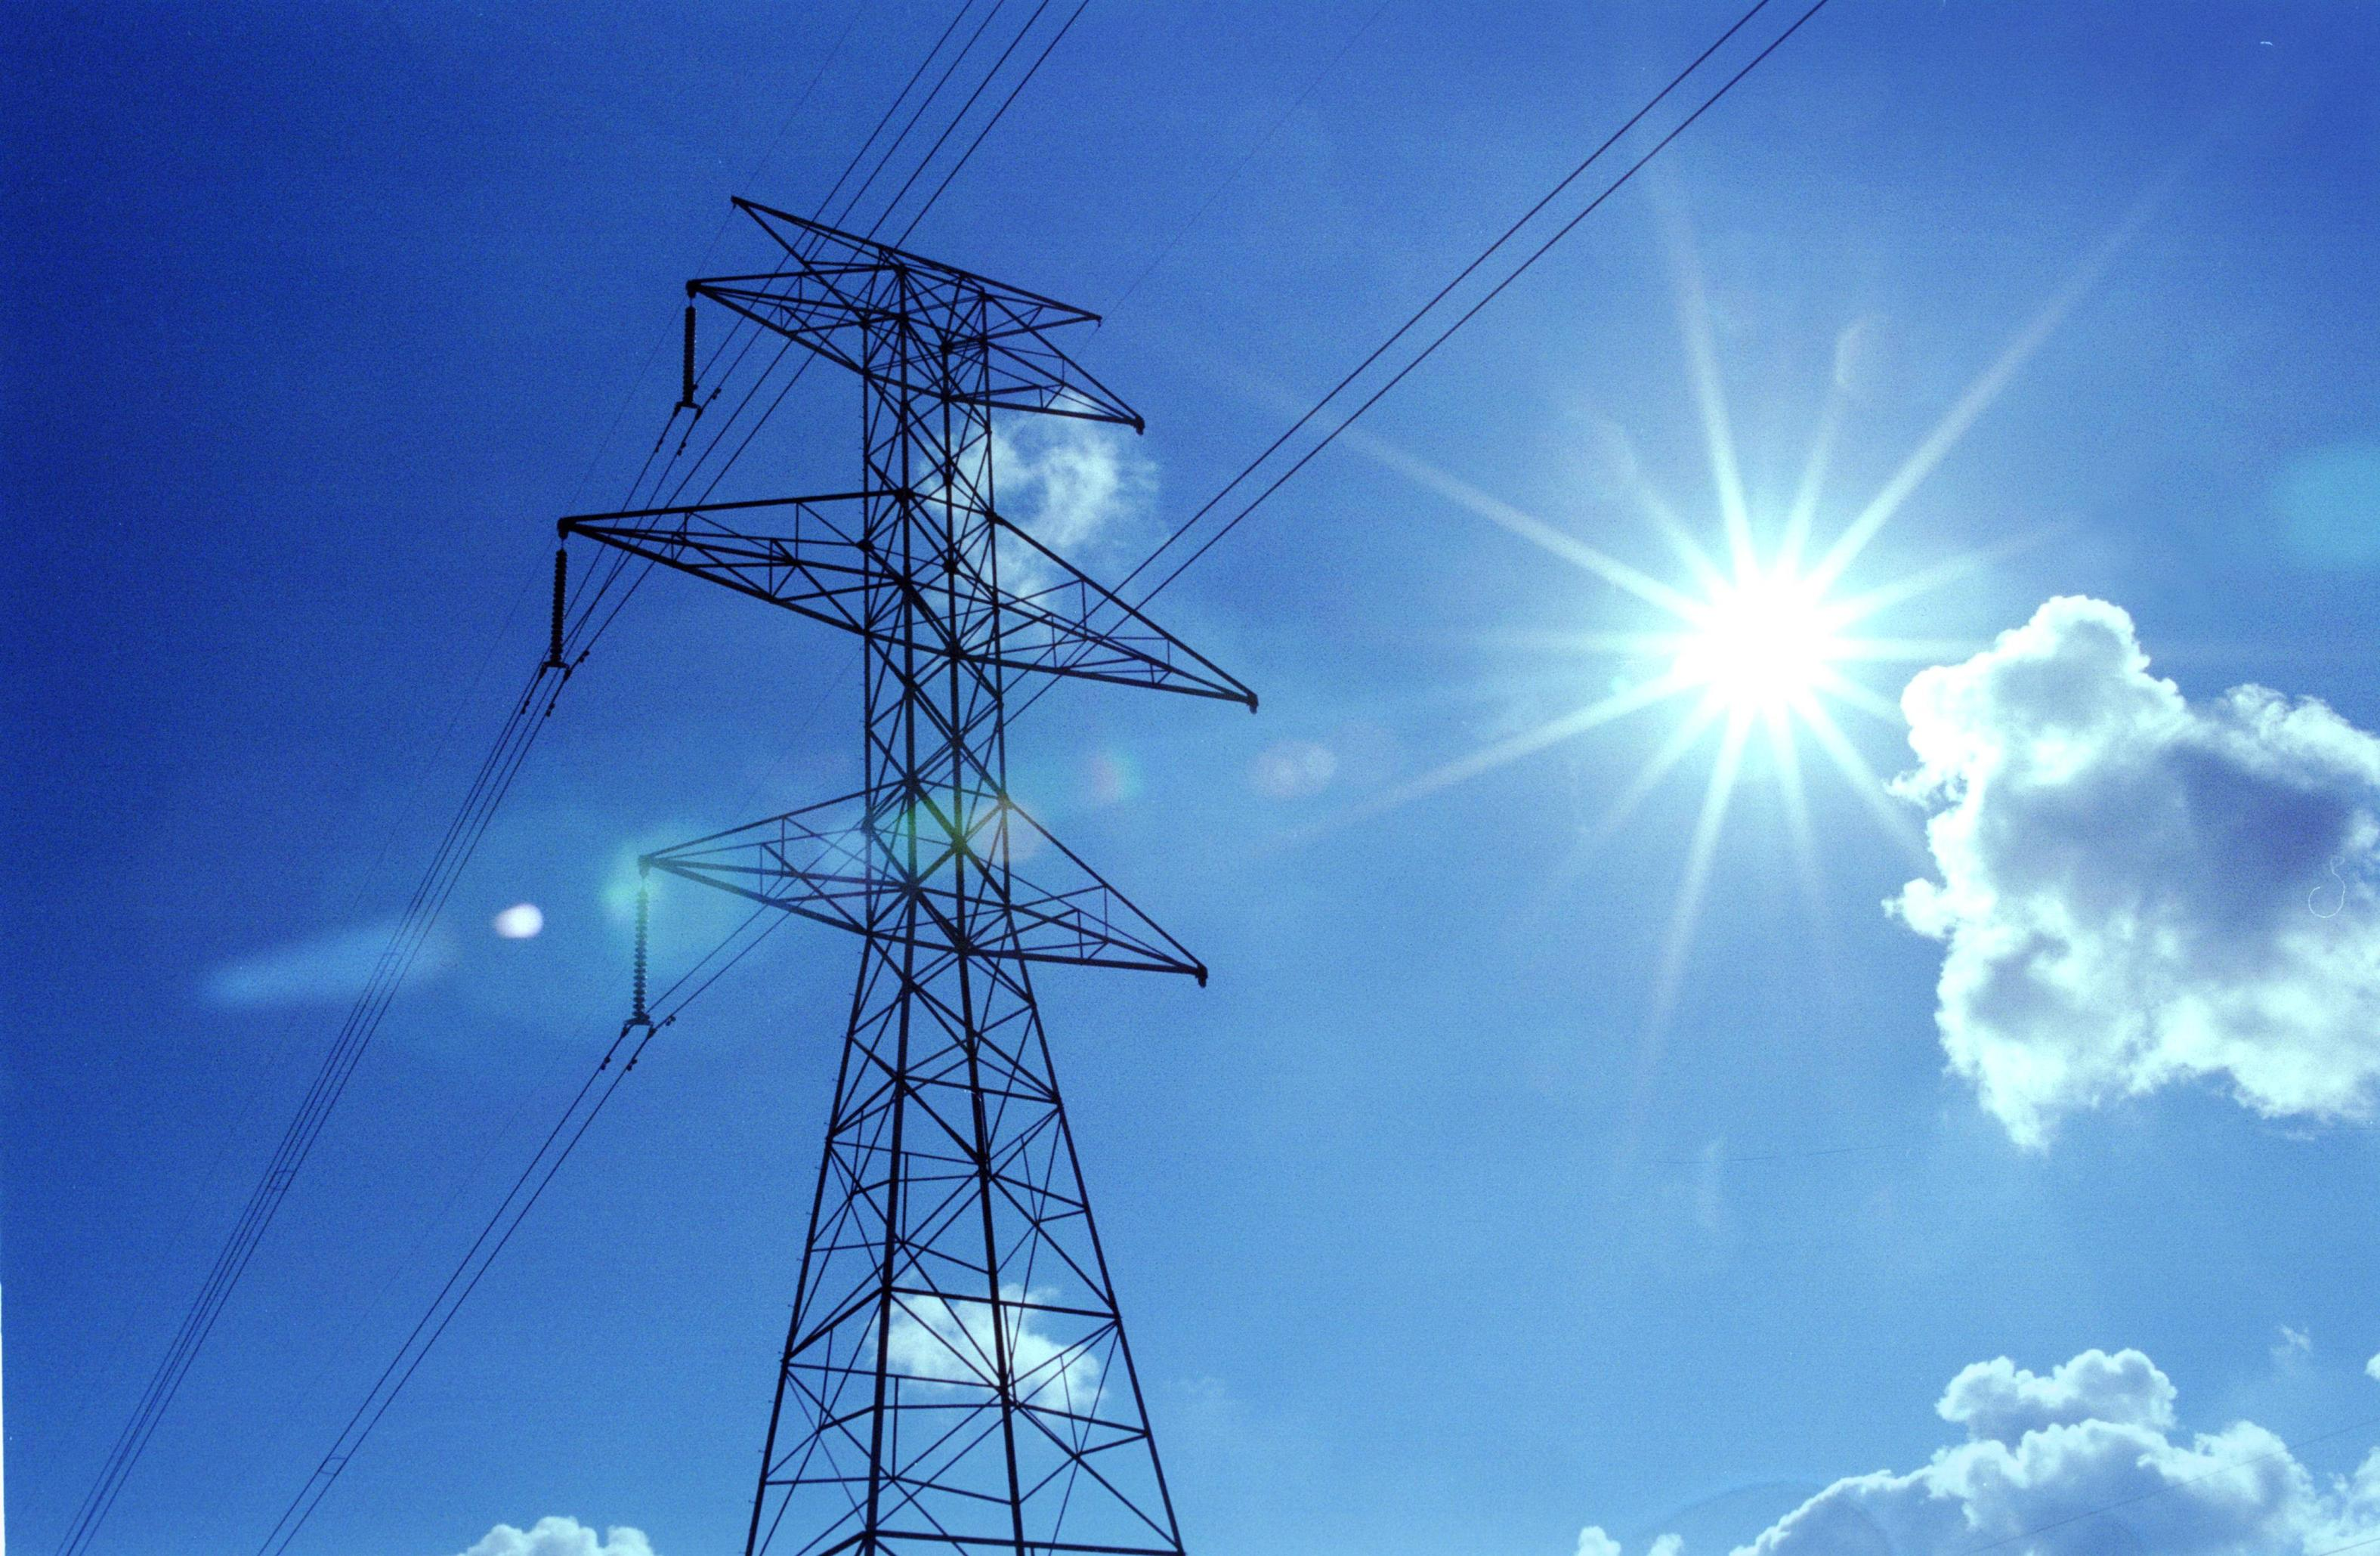
\includegraphics[width=1\linewidth]{\pathtopartone/graphics/transmission1}
\caption{Overhead transmission line}
\end{figure}

The concept of electromagnetic waves has fascinated man for so many years that man has asked so many questions varying from \emph{\textquotedblleft Why do stars twinkle?\textquotedblright}, to \emph{\textquotedblleft Why do magnetic needles deflect?\textquotedblright}, and \emph{\textquotedblleft how does light travel from the sun when there is no medium between?\textquotedblright}

In modern-day, questions vary from \emph{\textquotedblleft how do we have tv reception?\textquotedblright} to \emph{\textquotedblleft how do we have radio stations operating\textquotedblright} to \emph{\textquotedblleft how does a mobile phone work?\textquotedblright} to \emph{\textquotedblleft why are certain things heated when they are kept inside a microwave?\textquotedblright}. All these phenomena revolve around the concept of electromagnetic waves.\footnote{The concept of electromagnetic waves is virtually applied in almost all advanced technology.}

Electromagnetic waves can be divided into;
\begin{enumerate}[(i)]
\item low frequency and high power
\item high frequency and low power
\end{enumerate}

In this part of the book, we shall concentrate on the high-frequency and low-power properties of electromagnetic waves. Devices and phenomena like electrical machines, electrical power generators, transformers, and distribution of electrical energy fall into the category of low-frequency high power. Whereas modern systems, like mobile communication, radars, satellite, and optical fibres, fall into the high-frequency low-power category. So we are mainly going to investigate what happens as frequency increases in electromagnetic waves\footnote{
When the frequency of a wave increases, the wavelength will decrease to compensate for this increment
} and how they can be transmitted from one position to another without loss.

Electromagnetic waves see applications in many areas namely\footnote{
The applications of electromagnetic waves are not limited to this list but for this course, we streamline the application to these few.
}:
\begin{enumerate}[(i)]
\item Transmission lines and HF circuits.
\item Antennas.
\item Satellite communication.
\item Fibre-optic communication.
\item Radars.
\item Radio astronomy.
\item Electromagnetic Interference/Compatibility (EMI/EMC)
\end{enumerate}

We intend to investigate the behaviour of time-varying electric and magnetic fields especially when the frequency of operation is large. This investigation is going to be based on Maxwell's four equations of electromagnetic waves\footnote{
see \autoref{lec:lec18} for a detailed explanation of Maxwell's equations
}. However, as we proceed certain approximations can be used to investigate the same phenomena in terms of voltage and current which are electrical circuits.

\begin{figure}[h]
\centering
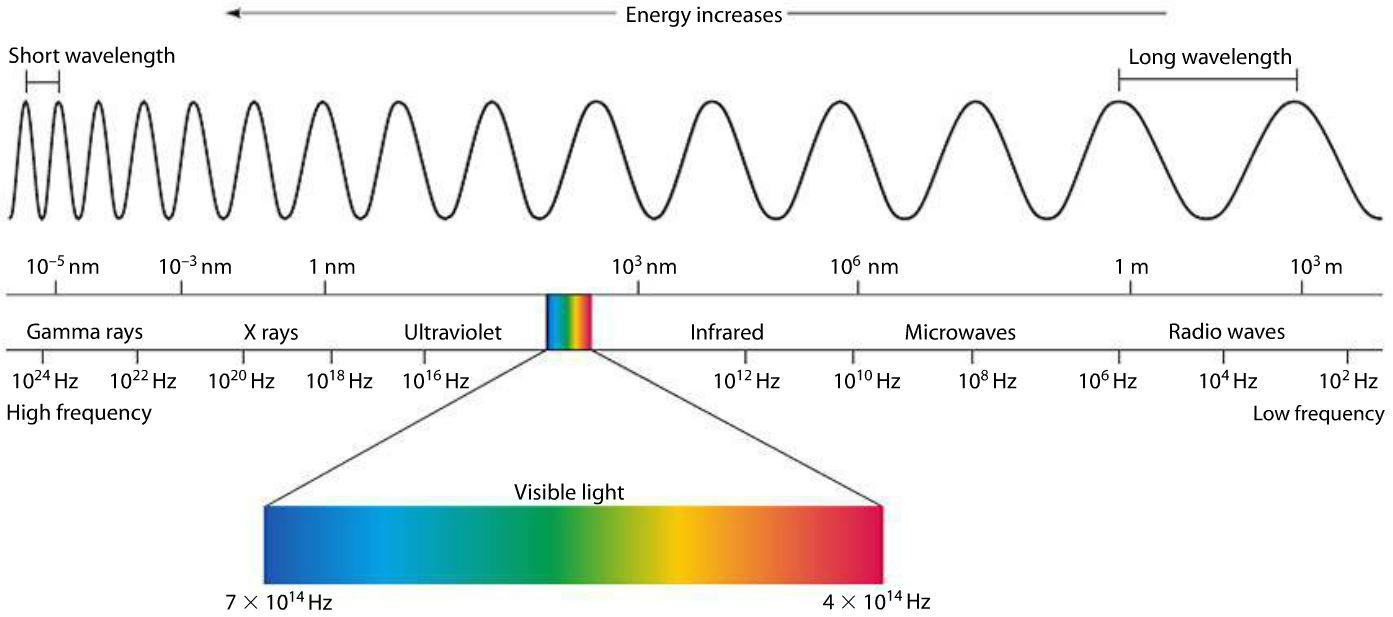
\includegraphics[width=1\linewidth]{\pathtopartone/graphics/electromagneticspectrum}
\caption{The electromagnetic spectrum}
\label{fig:electromagneticspectrum}
\end{figure}

\textbf{Electromagnetic spectrum:} All electromagnetic radiations in the universe ranging from very low frequencies to very high frequencies can be referred to as the electromagnetic spectrum. This is shown in figure~\ref{fig:electromagneticspectrum}

\section{Application of electromagnetic waves}
Depending on the frequency of operation, there are different media used to transmit electromagnetic waves. When the frequency is between 30MHz to 300MHz, the coaxial cable\index{coaxial cable} is used for transmission of the wave, from 30GHz to 300GHz the waveguide\index{waveguide} structure is used and as the frequency goes higher, the media used is the optical fibre\index{optic fibre}.

A question that comes to mind in electromagnetic wave transmission is \emph{\textquotedblleft Why do we have to increase frequency?\textquotedblright} \hspace{0.03in} To answer that we would have to think of the major application of high frequency which is in communication. Then for transmitting more information, we require large bandwidth. Since the frequency of operation is proportional to the bandwidth, by increasing the frequency of operation we increase the bandwidth and as such one can transmit more information on a given channel.

\subsection{Transmission Line}
\begin{figure}[h]
\centering
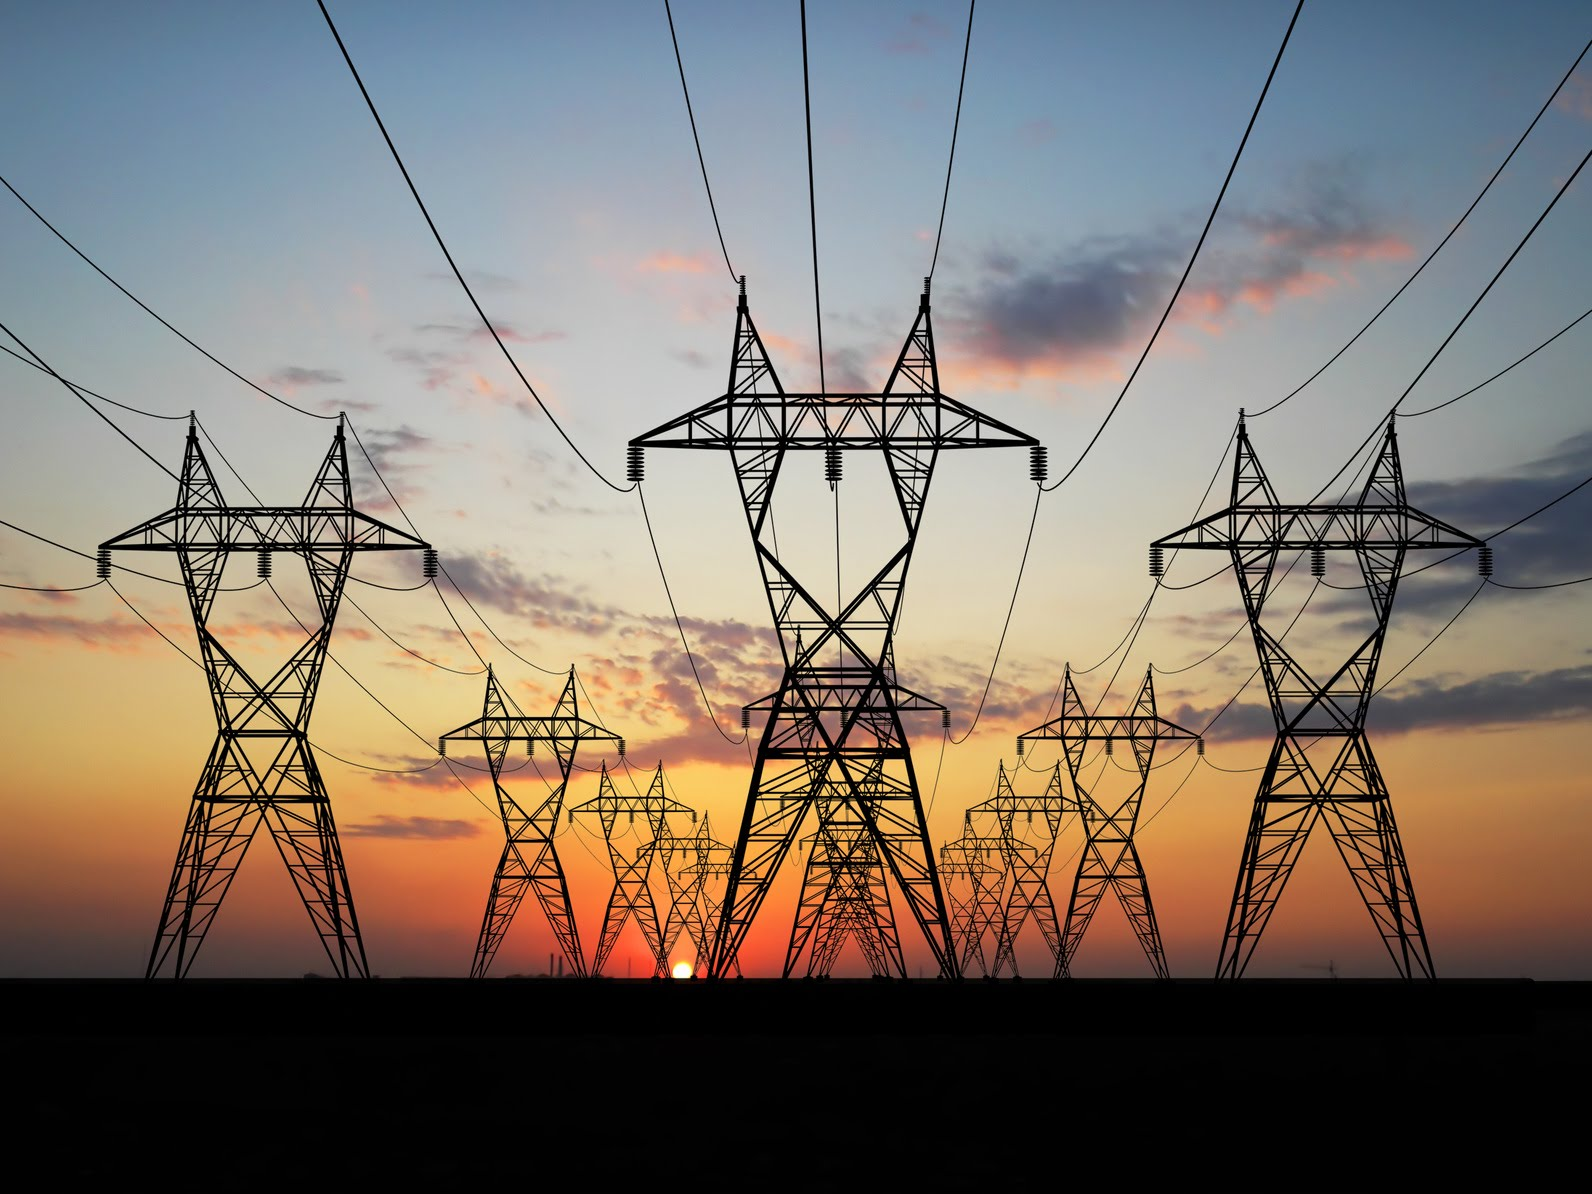
\includegraphics[scale=0.1]{\pathtopartone/graphics/transmission2}
\caption{Power transmission line}
\end{figure}

In transmission lines, our main concern is how voltage and current would flow in a two-conductor system called a \textit{transmission line} and how losses occur during transmission \footnote{
When the frequency of a wave increases its wavelength decreases and when the wavelength of the wave is comparable to the length of the transmitting media (length of the wire) the losses along the wire become too significant to ignore.
}.

There are different types of transmission media and the application of this media is based on the frequency range of the signal.
\begin{figure}[h]
\centering
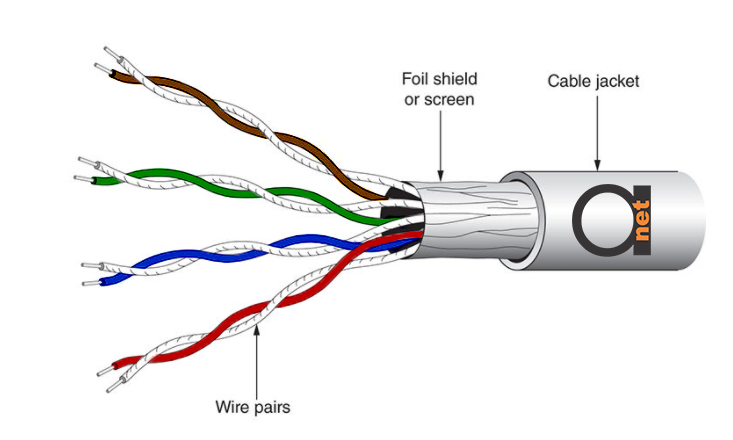
\includegraphics[width=1\linewidth]{\pathtopartone/graphics/twistedpairs}
\caption{Twisted pair of wires}
\end{figure} 

\subsubsection{Twisted pairs}
They are point-to-point transmission lines\footnote{
Connections between two nodes or endpoints
} (it is a balanced transmission line having voltages $v^{+}$ and $v^{-}$ connected at its terminals). An example of the twisted pairs is the telephone wires; it is characterized by low data rate, high Electromagnetic Interference (EMI)\index{electromagnetic interference} and is lossy at radio frequencies.

\subsubsection{Coaxial cable}
For the coaxial cable, we have an example in the LAN (Local Area Network) cable; it characterizes data rates of up to a few Mbps, low EMI and moderate loss.
\begin{figure}[h]
\centering
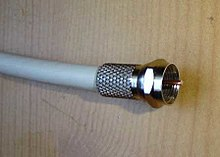
\includegraphics[scale=0.5]{\pathtopartone/graphics/coaxialcable}
\caption{Coaxial cable}
\end{figure}

\subsection{Waveguides}
These are hollow circular or rectangular pipes and they are used when the frequency becomes high in other to reduce losses. 

Inside the hollow metal conductor, an electromagnetic wave can propagate and here rigorous analysis of electromagnetic wave propagation is carried out to help find out what the field distribution would look like and how much energy loss will take place inside.
\begin{figure}[h]
\centering
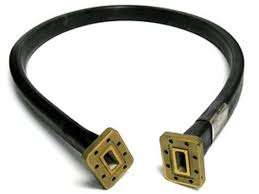
\includegraphics[scale=0.5]{\pathtopartone/graphics/waveguide2}
\caption{Waveguide\index{waveguide}}
\end{figure}

\subsection{Antennas}
\begin{figure}[h]
\centering
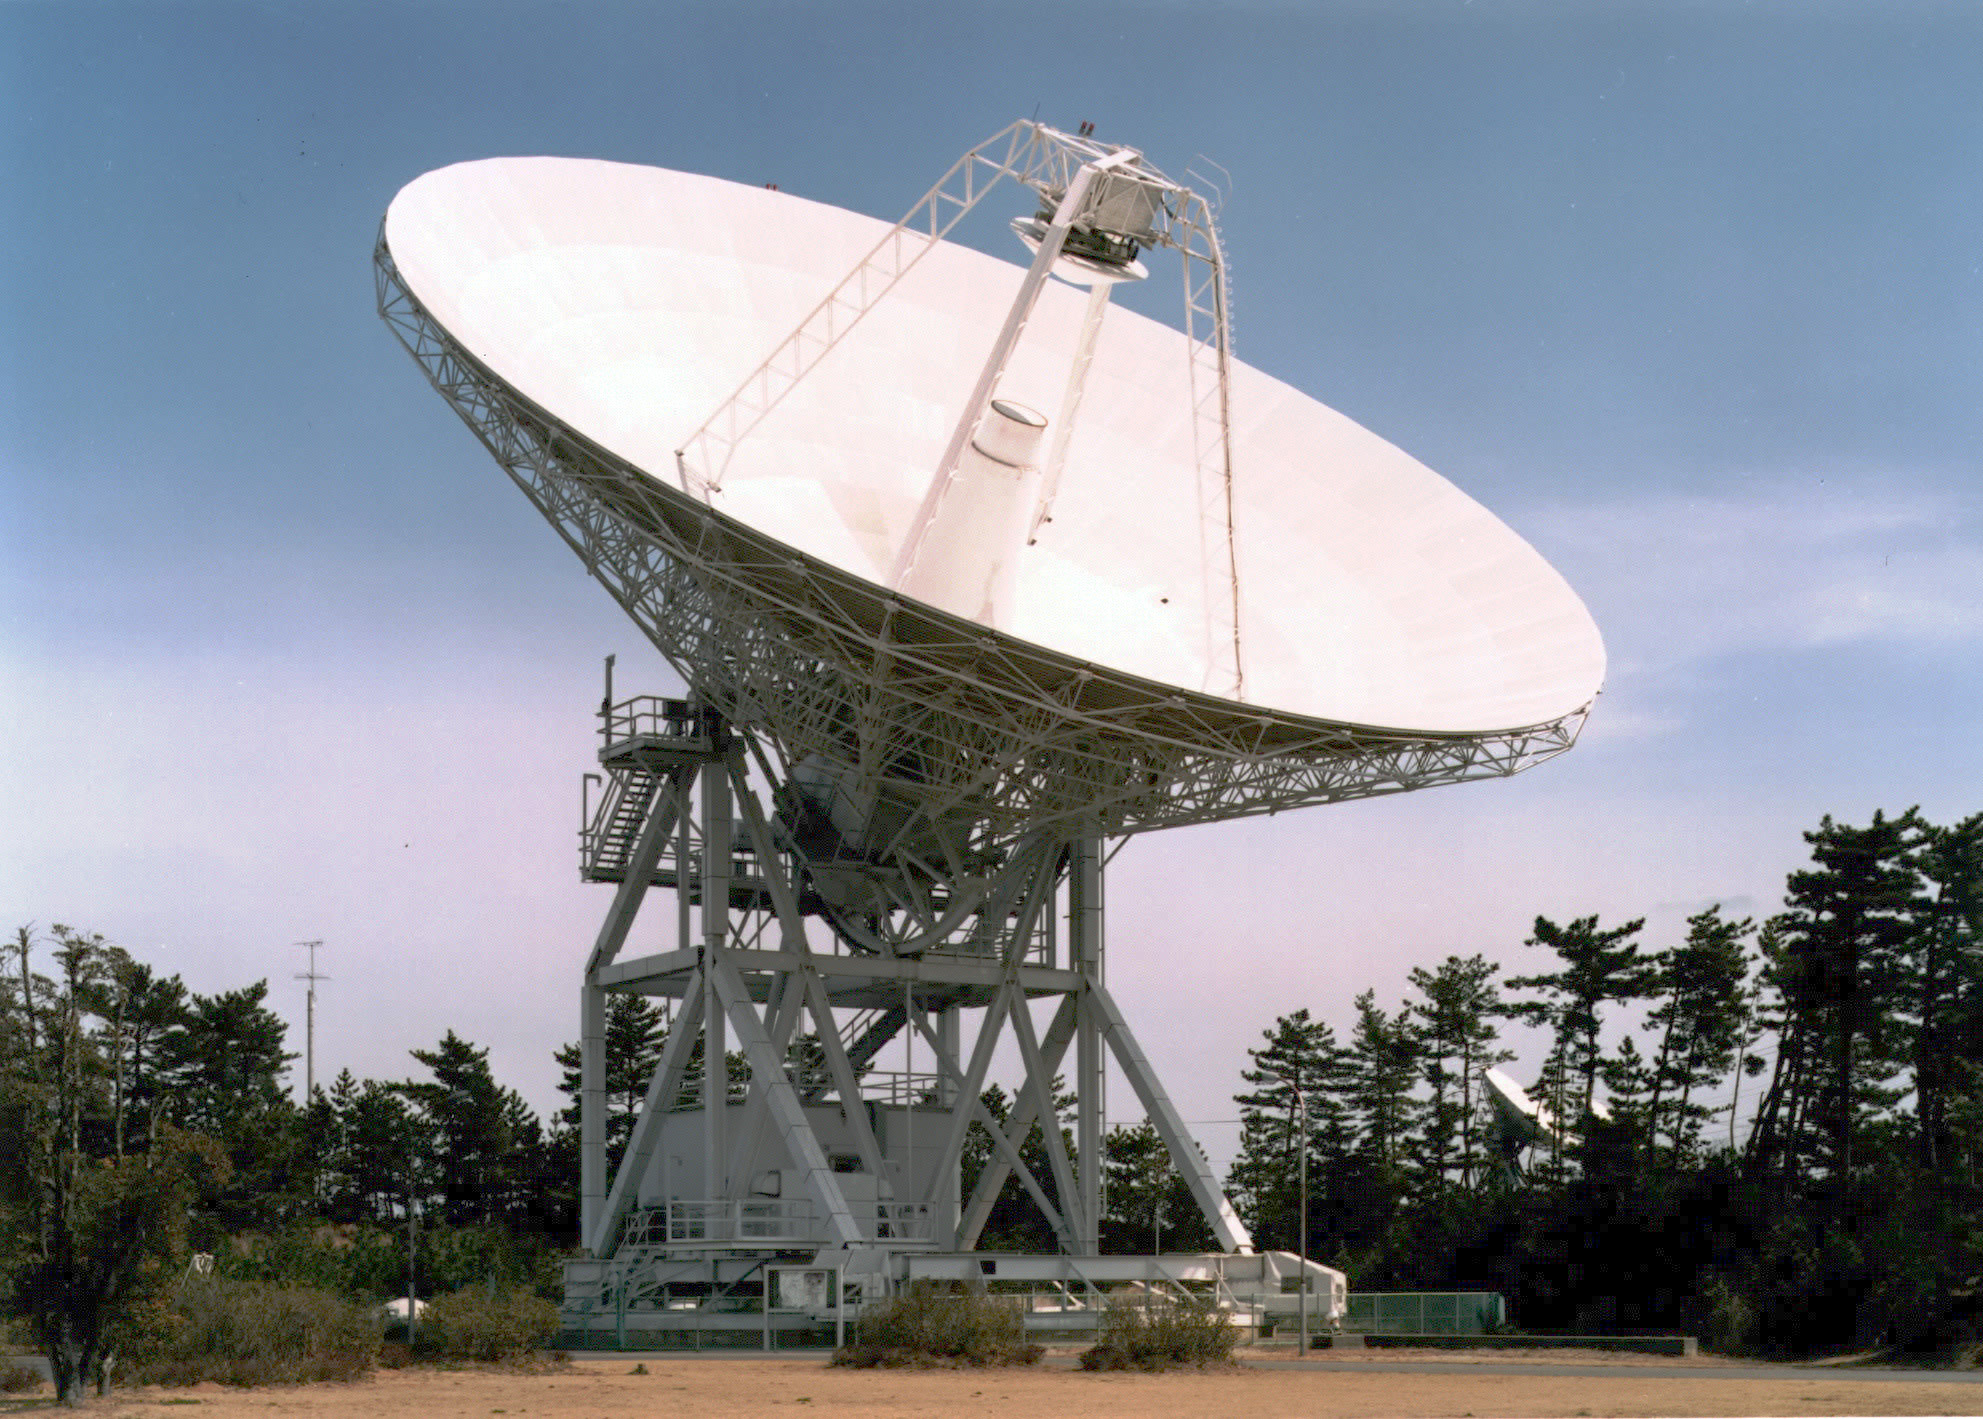
\includegraphics[scale=0.4]{\pathtopartone/graphics/spcaceantenna}
\caption{Parabolic dish antenna}
\label{fig:spaceantenna}
\end{figure}

An antenna is a device that can transmit electromagnetic energy into space and also can receive electromagnetic energy coming from space. An example is the parabolic dish antenna (see figure~\ref{fig:spaceantenna}), signals coming from a point are like parallel rays. When it gets to the parabolic dish antenna the rays converge to a focal point called the feed from there they get processed into an electrical signal.

An antenna is a device that separately puts radiation in the desired direction. A simple antenna structure may not necessarily provide the desired characteristics of modern-day smart antenna systems where radiation characteristics can be automatically changed to maximize the reception of the signal.

Other more advanced antenna systems referred to as \textbf{smart antennas} can selectively steer the radiation in the desired direction. There are two types of smart antennas which are the \textbf{adaptive array} and \textbf{switched beam systems}.

\subsubsection{Adaptive array\index{adaptive array antenna}}
They steer the beam in the direction of the user/observer while simultaneously nulling interfering signals (see figure~\ref{fig:fh06_02}).
\begin{figure}[h]
\centering
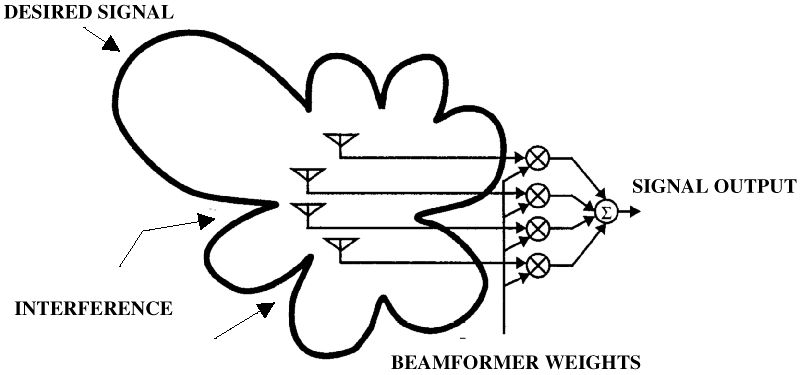
\includegraphics[scale=0.3]{\pathtopartone/graphics/fh06_02}
\caption{Adaptive array system}
\label{fig:fh06_02}
\end{figure}

\subsubsection{Switched beam antenna\index{switched beam antenna}}
It has multiple beams (see figure~\ref{fig:switchedbeam}) which can be switched depending on the area an observer is situated so that a signal can be transmitted or received from that zone. Therefore, depending on the requirement of the system a beam is selected hence the name switched beam.
\begin{figure}[h]
\centering
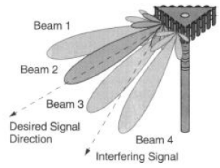
\includegraphics[scale=0.7]{\pathtopartone/graphics/switchedbeam}
\caption{Illustration of a switched beam antenna}
\label{fig:switchedbeam}
\end{figure} 


\subsection{Satellite communication}\index{satellite communication}
A satellite is an object that is placed above the earth's surface. There is a satellite station on the earth's surface usually called the earth station which transmits signals from the earth to satellites and also receives signals from satellites to the earth. With satellite communication there are certain frequency bands are assigned. Satellite communication is a point-to-multi-point system.

\begin{figure}[h]
\centering
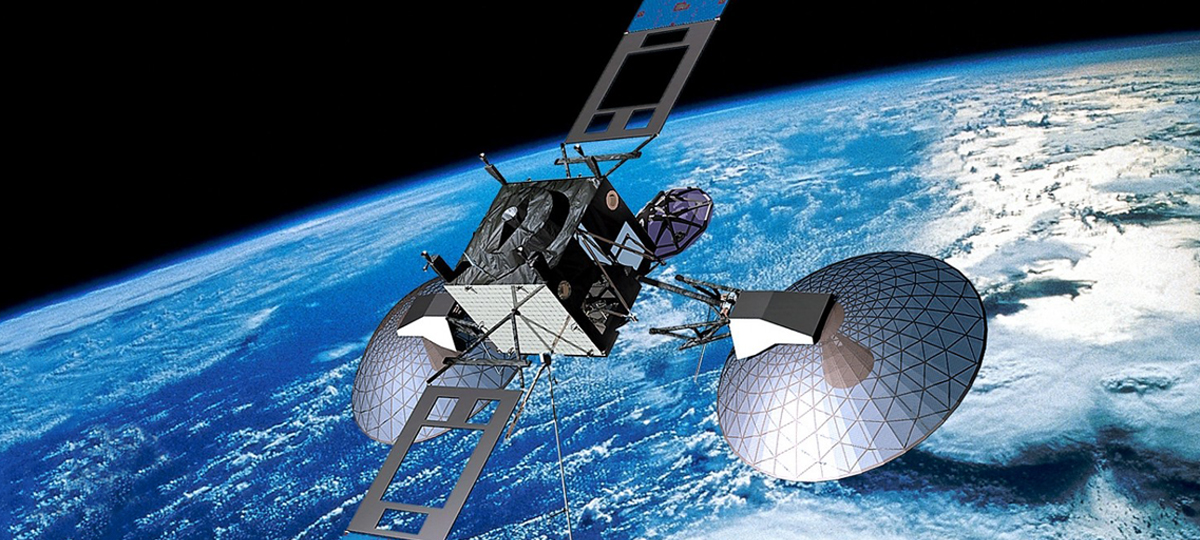
\includegraphics[scale=0.2]{\pathtopartone/graphics/satellite}
\caption{Space satellite}
\end{figure}

The whole propagation of the electromagnetic wave and proper placing of radiation in the direction towards the earth is achieved using the principles of electromagnetic waves. Satellite communication has a large time delay because of the turnaround trip time taken from the Earth station to the satellite and from the satellite back to the Earth station.

\subsection{Fiber optics communication}
\begin{figure}[h]
\centering
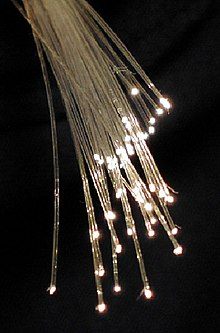
\includegraphics[scale=0.4]{\pathtopartone/graphics/opticalfiber1}
\caption{Optical fiber}
\label{fig:opticalfibre1}
\end{figure}

Knowledge of electromagnetic waves is required to investigate the propagation of light inside a fibre optic material. A fibre optic cable\index{fibre optic cable} (see figure~\ref{fig:opticalfibre1}) is made up of very thin hollow glass strands in which light is reflected internally. As the light propagates inside the optical fibre, the signal gets distorted and hence the knowledge of electromagnetic waves is needed to know how the signal gets distorted.

\subsection{Wireless communication}
Wireless communication is used in cell phones and most modern systems like home entertainment systems using Bluetooth speakers, laptops using a wireless method to connect to routers and so on. All these work on the principle of electromagnetic waves.
\begin{figure}[h]
\centering
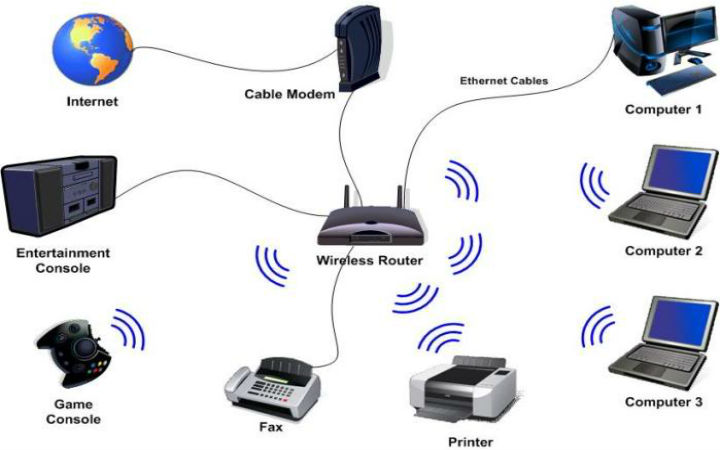
\includegraphics[scale=0.3]{\pathtopartone/graphics/Expert-support-for-wireless-communication-projects}
\caption{Wireless connection of devices}
\end{figure}

\subsection{Cellular communication} 
In cellular communication, we have the base station from where the signals are transmitted, all users located inside are called a cell (see figure~\ref{fig:rrsadafig1}). Any mobile call made goes from the handset to the base station in that sector and then goes to the desired handset within the same sector or in another sector.
\begin{figure}[h]
\centering
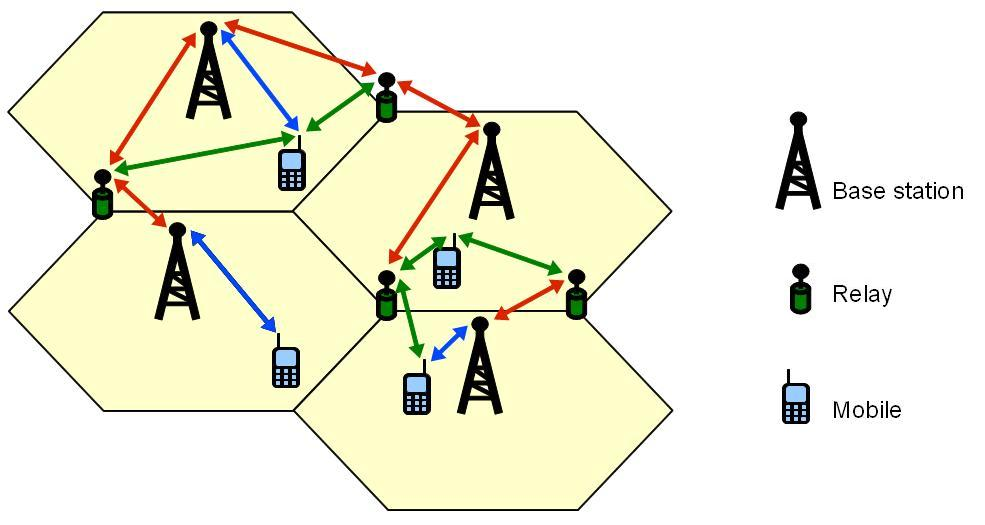
\includegraphics[scale=0.3]{\pathtopartone/graphics/RR_sada_fig1}
\caption{Cellular communication}
\label{fig:rrsadafig1}
\end{figure}

It is observed that a cell phone user has signals from multiple paths all coming to his cell phone\footnote{Wireless relays are used to transmit and receive information between the base station and mobile when they are too far away to send the information to each other directly}. The mobile entity does not only get signals coming directly from the base station, but it also encounters signals due to reflection from associated objects. As a result of interference of these signals which can either be constructive or destructive, the final signal transmitted/received is altered (see figure~\ref{fig:rod}). 

When there is constructive interference, a strong signal strength is observed and when the interference is destructive, a weak signal strength is observed. The gradual weakening of a signal due to destructive interference is called \textit{fading}\index{fading}. To understand fading phenomenon a good knowledge of electromagnetic waves is required. To avoid fading phenomena, antennas in mobile phones use \textit{sectioned radiation patterns}\index{sectioned radiation patterns}. This implies that the cell phone gets its signal from the base station directly while minimizing signals from paths not in the direction of the base station of the antenna. A good knowledge of electromagnetic waves is required to design such antennas.
\begin{figure}[h]
\centering
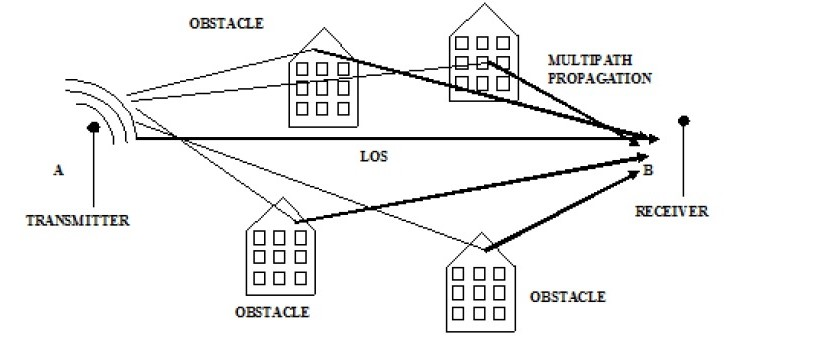
\includegraphics[scale=0.4]{\pathtopartone/graphics/rod}
\caption{Illustration of signal inference}
\label{fig:rod}
\end{figure}

\subsection{Radar and remote sensing}
In radar altimetry, electromagnetic waves are used for finding the distance of an object from its position in space to the antenna. The antenna is excited with an electromagnetic pulse and the dish beams parallel waves downwards. This beam is reflected from the earth's surface/target object back to the dish. The dish converges the received signal back to the antenna and processes it in the detector (see figure~\ref{fig:new}).
\begin{figure}[h]
\centering
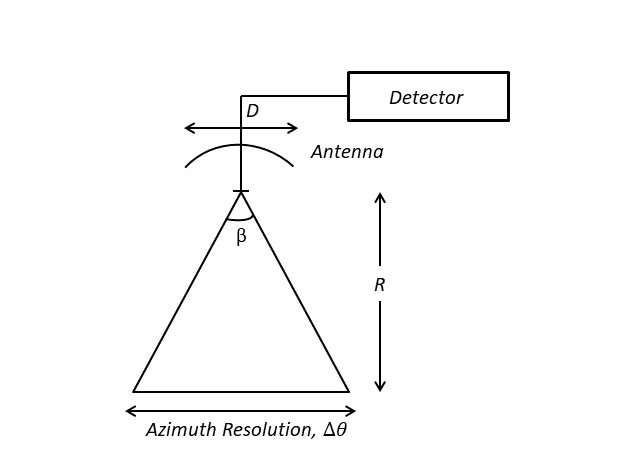
\includegraphics[width=1\linewidth]{\pathtopartone/graphics/Azimuth_resolution}
\caption{Illustration of Azimuth resolution}
\label{fig:new}
\end{figure}

The \textit{Azimuth (or bearing) resolution}\index{azimuth resolution} of the radar is given as $\Delta \theta = \beta R = \frac{\lambda R}{D}$\footnote{The implication of this equation lies in the size of the antenna. To get a high resolution the size of the antenna would be large}, where $\beta$ is the beam width of the antenna given as $\dfrac{\lambda}{D}$, $\lambda$ is the wavelength of the beam, $R$ is the range of distance covered by the beam and $D$ is the aperture of the antenna. It is the measure of the ability of an imaging radar to separate two closely spaced scatterers in the direction parallel to the motion of the beam (resolution at the same range but different bearings). Similarly, the measure of the ability of a radar to correctly resolve the position of two closely spaced objects in the range is called the \textit{range resolution}\index{range resolution} which makes up the second category of resolution in radar systems. It is given as $\geq \dfrac{cT}{2}$ where $c$ is the speed of light, and $T$ is the transmission pulse width.

With radar systems, the distance travelled by the beam can be estimated and also if the object is moving in the radial direction, there would be a frequency change between the signal transmitted by the antenna and the signal reflected (Doppler shift) and from this result the velocity of the object can be estimated. The radar essentially uses the electromagnetic pulse to find the distance and the velocity of an object.

\subsubsection{The monostatic radar equation}
\begin{figure}[h]
\centering
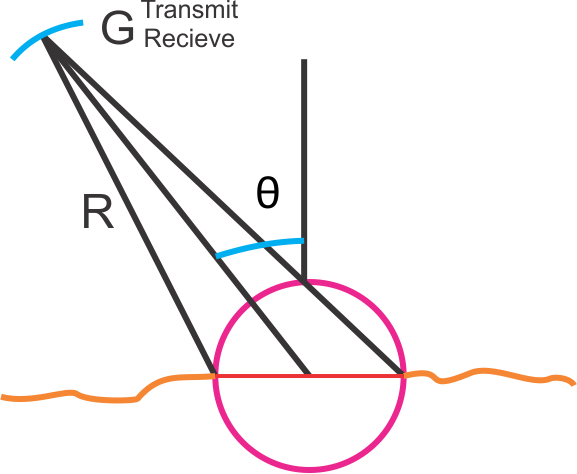
\includegraphics[width=.8\linewidth]{\pathtopartone/graphics/new1}
\label{fig:new1}
\caption{Illustration of the monostatic radar equation}
\end{figure}

The monostatic radar equation is given as
\begin{dmath*}
P_{r}= \frac{P_t G\sigma A}{(4\pi)^{2}R^{2}}
\end{dmath*}
$P_{r}$ is the received power, $P_t$ is the transmitted power, $G$ is the antenna gain, $\sigma$ is the radar cross section of the target, $A$ is the effective area of the antenna and $R$ is the range(see  figure~\ref{fig:new1}). The signal goes from the radar transmitting antenna to the object and is again received by the receiving antenna in the radar. The magnitude of the received signal can be calculated and this requires a good knowledge of the ability to model the propagating environment and a good modelling of the scatterer from which the energy is going to be reflected.

\begin{figure}[h]
\centering
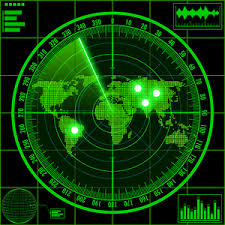
\includegraphics[scale=0.5]{\pathtopartone/graphics/radarlocator}
\caption{Radar locator}
\label{fig:radarlocator}
\end{figure}

Figure~\ref{fig:radarlocator} depicts a radar locator. We can see the various objects detected by the radar (represented by the white dots) and the green radial line represents the transmitting beam

\subsubsection{Side looking airborne radar (SLAR)} 
It is a radar technique used for remote sensing. It is an imaging radar\footnote{Imaging radar provides its light to illuminate an area on the ground and takes the picture at radio wavelengths} mounted on a moving object like an aircraft, pointing perpendicular to the direction of flight (hence side-looking). A squinted (non-perpendicular) mode is possible also. SLAR can be fitted with a standard antenna (real aperture radar) or an antenna using synthetic aperture(this would be discussed in the next section). The platform of the radar moves in the direction of the x-axis. The radar looks with the looking angle $\theta$ (or so-called off-nadir angle).

The microwave beam is transmitted obliquely at right angles to the direction of flight illuminating a swath (see figure~\ref{fig:slar2}). \textit{Swath width}\index{swath width} refers to the strip of the earth's surface from which data are collected by a side-looking airborne radar. It is the width of the imaged scene in the range dimension. The longitudinal extent of the swath is defined by the motion of the aircraft with respect to the surface, whereas the swath width is measured perpendicularly to the longitudinal extent of the swath. Range refers to the across-track dimension perpendicular to the flight direction, while azimuth refers to the along-track dimension parallel to the flight direction\footnote{This technique is mostly used in aircraft}.

\subsubsection*{To measure the azimuth resolution}
The SLAR is primarily a real aperture radar. This requires a reasonably large antenna for adequate angular resolution. The azimuth resolution, $ Ra $, is defined as

\begin{center}
$R_{a}=\frac{H \lambda}{D cos\theta}$
\end{center}
$ H $ is the height of the antenna(height of the airplane)\\
$ D $ is the geometric length of the antenna,\\
$\lambda$ is the wavelength of the transmitted pulses, and\\
$\theta$ is the incidence angle

\begin{figure}[h]
\centering
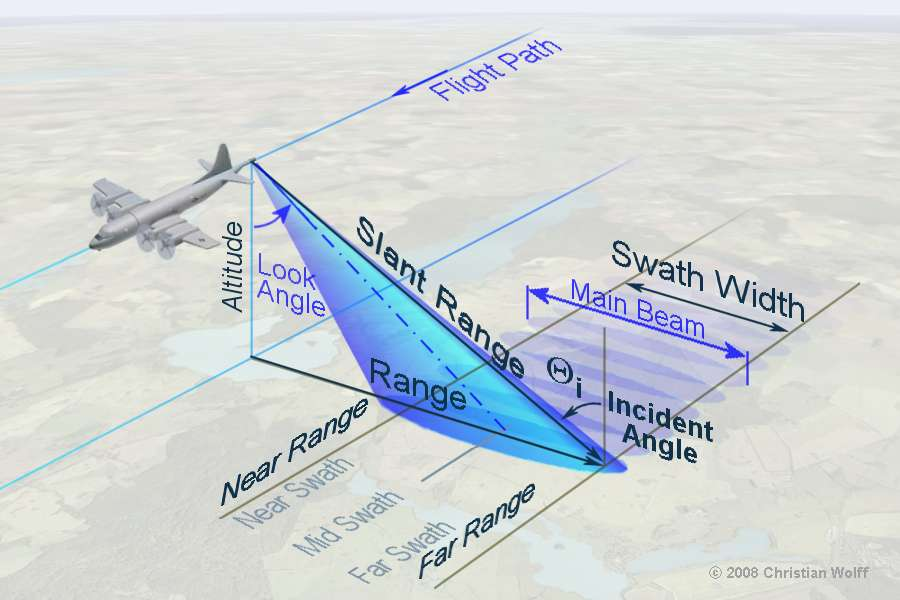
\includegraphics[width=.8\linewidth]{\pathtopartone/graphics/SLAR2}
\caption{Diagram of the SLAR}
\label{fig:slar2}
\end{figure}

The equation shows, that increasing altitude decreases the azimuthal resolution of SLAR. A very long antenna (i.e., large D)\footnote{For this book, $D$ is the size of the antenna. hence the statement \textquotedblleft large D\textquotedblright\; since the length ($L$) of an object is a function of the size ($D$)} would be required to achieve a good resolution from the aircraft. Synthetic Aperture Radar (SAR) is used to acquire higher resolution.

\subsubsection{To measure the cross-track resolution}
At all ranges, the radar antenna measures the radial line of sight distance between the radar and each target on the surface. This is the slant range distance. The ground range distance is the true horizontal distance along the ground corresponding to each point measured in the slant range. The cross-track resolution, $R_{r}$, is defined as:  
\begin{center}
$R_{r}=\frac{c_{0} t_{p}}{2 sin\theta}$
\end{center}
$c_{0}$ is the speed of light\\
$t_{p}$ is the pulse duration of the transmitter and\\
$\theta$ is the incidence angle

\subsubsection{To measure the cross-track resolution}
At all ranges, the radar antenna measures the radial line of sight distance between the radar and each target on the surface. This is the \textit{slant range}\index{slant range} distance. The ground range distance is the true horizontal distance along the ground corresponding to each point measured in the slant range. The \textit{cross-track resolution}\index{cross-track resolution}, $R_{r}$, is defined as:  
\begin{dmath*}
R_{r}=\frac{ct_{p}}{2\sin\theta}
\end{dmath*}
$c$ is the speed of light, $t_{p}$ is the pulse duration of the transmitter and $\theta$ is the incidence angle
\begin{figure}[h]
\centering
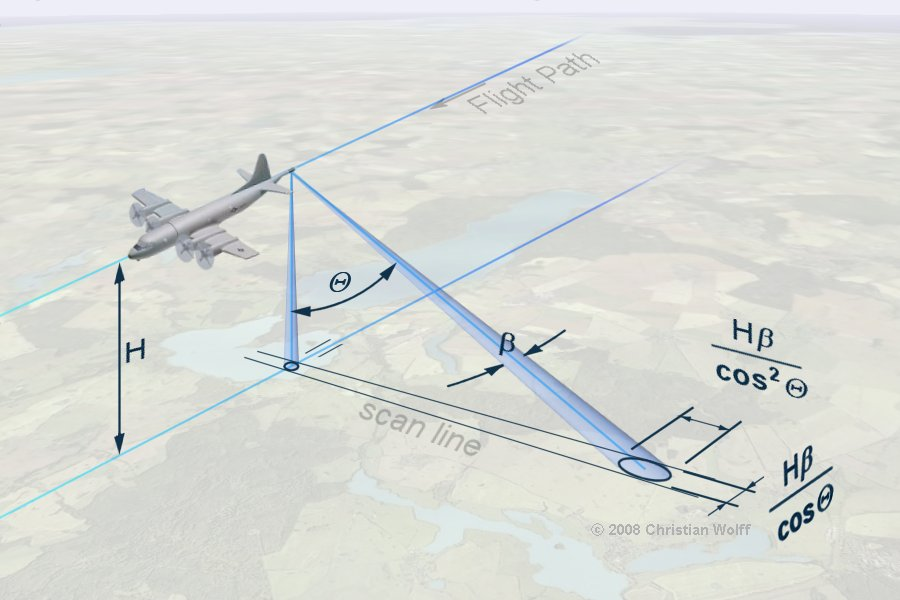
\includegraphics[width=1\linewidth]{\pathtopartone/graphics/fig 1.19(SLAR)}
\caption{Diagram of the SLAR}
\end{figure}

\subsubsection{Synthetic aperture radar(SAR)}
To improve the resolution in remote sensing, a technique called the synthetic aperture dish is used. For an antenna like a parabolic dish, the angular resolution is given as the wavelength divided by the size\footnote{For a parabolic dish antenna the diameter \textquotesingle d\textquotesingle is used instead of length \textquotesingle L\textquotesingle. See footnote 11} for the antenna, $\Delta \theta = \frac{\lambda}{D}$. To get a fine resolution for the image in remote sensing, a very large aperture D is required. A large D cannot be easily created especially in moving vehicles and aircraft.\\

\subsubsection{Synthetic aperture radar (SAR)}
To improve the resolution in remote sensing, a technique called the \textit{synthetic aperture dish} is used. For an antenna like a parabolic dish, the angular resolution is given as the wavelength divided by the size (or aperture)\footnote{For a parabolic dish antenna the diameter \textquotedblleft d\textquotedblright \hspace{0.02in} is used instead of length \textquotedblleft L\textquotedblright. See \autoref{fn:fn1}} for the antenna $\Delta \theta = \frac{\lambda}{D}$. To get a fine resolution for the image in remote sensing, a very large aperture $D$ is required. A large $D$ cannot be easily created especially in moving vehicles and aircraft.

To mitigate this, there is a technique where the antenna is small but the vehicle moves and as the vehicle moves, the reflection information is stored after all the refection information is collected from different locations, then data processing can be done to get an angular resolution which will correspond to the total distance travelled by the vehicle. This technique is known as the \textit{synthetic aperture radar}\index{synthetic aperture radar} (see figure~\ref{fig:sar2}).
\begin{figure}[h]
\centering
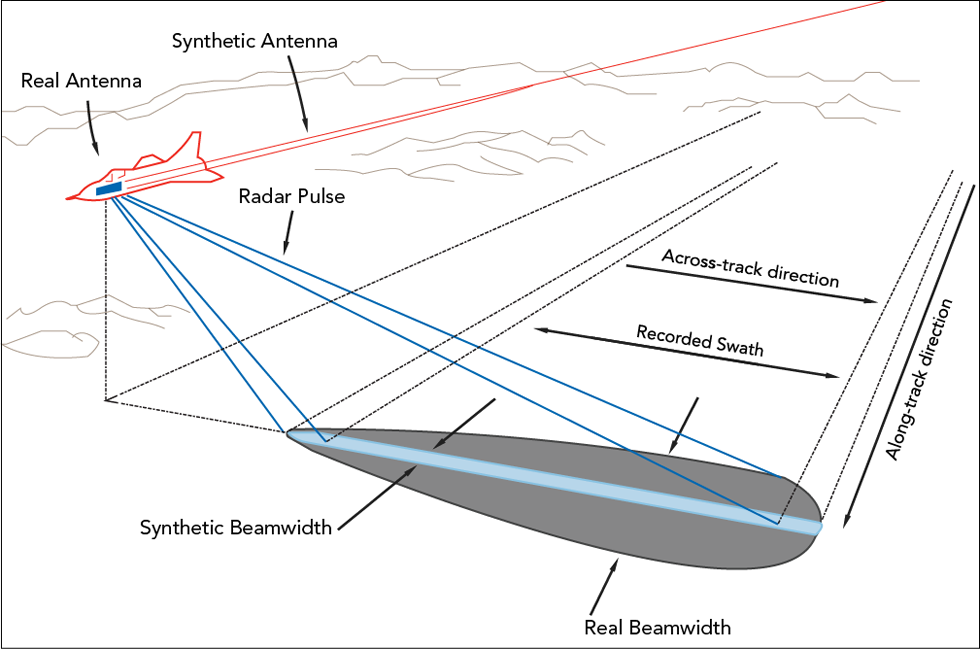
\includegraphics[scale=0.35]{\pathtopartone/graphics/sar2}
\caption{Diagram illustrating the SAR}
\label{fig:sar2}
\end{figure}

\subsubsection*{Features of the SAR}
\begin{enumerate}[(i)]
\item It has a very high linear resolution independent of the range
\item It requires a source with higher coherence
\item The image is on the range-doppler coordinate grid
\item It requires a large data processing
\item There are geometric and ratio metric distortions
\item There is speckle noise in the image
\end{enumerate}

\subsection{Radio astronomy} 

A typical radio telescope is shown in figure~\ref{fig:radiotelescope0} with a passive receiver. In this case, no signal is transmitted but the signal is received.
\begin{figure}[h]
\centering
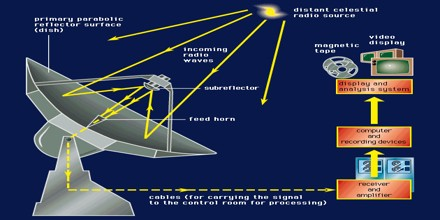
\includegraphics[scale=0.5]{\pathtopartone/graphics/Radio-Telescope-0}
\caption{Radio telescope}
\label{fig:radiotelescope0}
\end{figure}

The frequency of the signals is converted, detected and processed. With a radio telescope, we would like to get an image of the sky with as large a resolution as possible.

$\frac{\lambda}{D}$ comes into the picture and to get a very fine resolution of the image of the sky, a very large telescope would be needed.


Producing a very large telescope is difficult so we use the synthetic aperture technique as it was used on radars. In this method, we use a set-up of antennas, for example, if the dish in each array is of the order of $ D = 25m $ and the total spread of the antennas of the order 21km. Therefore, we get an effective aperture through each antenna that has an aperture of only 25m.

\subsection{EMI/EMC}

\textbf{EMI} is \textit{electromagnetic interference}\index{electromagnetic interference}. Firstly, let us investigate how a high-frequency device would create interfering signals and then what ways in which the interference can be reduced.

For example, you may get interference on our radios, whenever somebody starts a car or a motorcycle in the vicinity because starting a car or motorcycle involves sparking and because of that spark, you get electromagnetic interference which is picked up by the radio antenna and you get disturbance on your radios. It is essential to investigate the technique by which the interferer can be reduced or the mechanism by which the devices can be isolated. This technique is called \textit{\textbf{shielding}}.

\textbf{EMC} is electromagnetic compatibility. Today, whenever we design electromagnetic gadgets or electrical devices it is mandatory to make them electromagnetically compliant so it does not create additional electromagnetic interference which will affect other systems.

The figure below describes the whole concept of EMC, illustrating both causes(natural or man-made) and solutions (shielding and other techniques).

\begin{figure}[h]
\centering
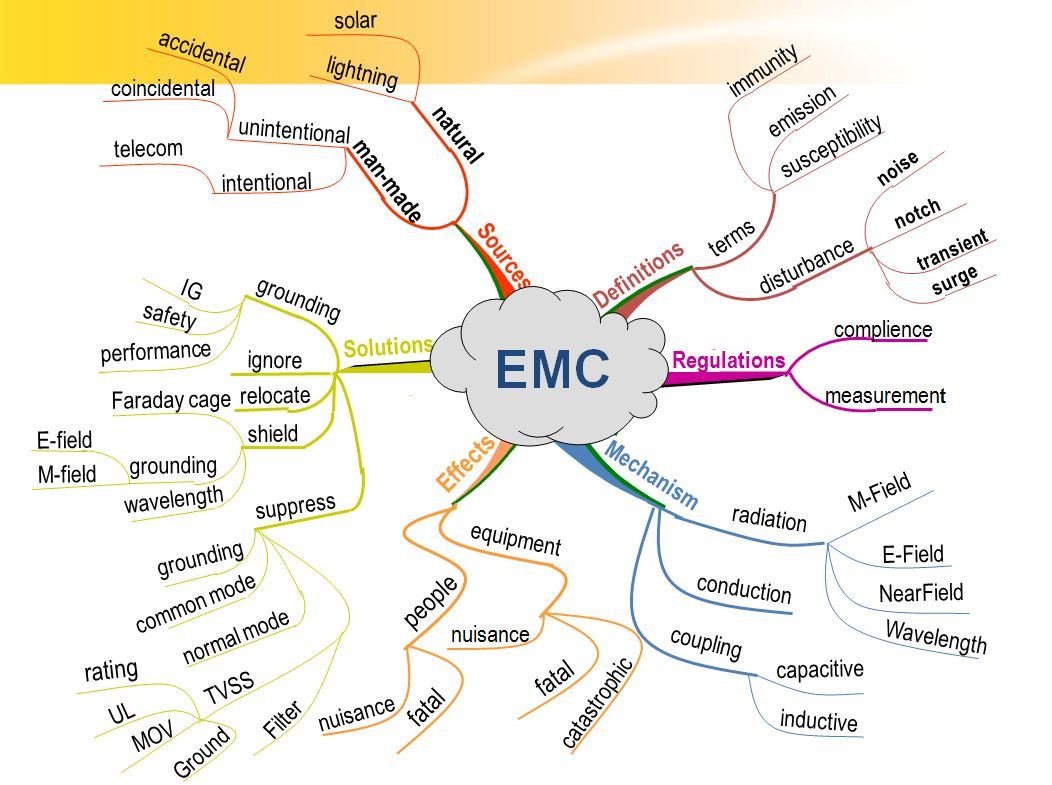
\includegraphics[scale=0.35]{\pathtopartone/graphics/634771461726914062}
\caption{Electromagnetic Compatibility}
\label{fig:634771461726914062}
\end{figure}

\newpage
\section*{Exercises}
\begin{ExerciseList}
\Exercise[label={ex11}]
What is the difference between adaptive arrays and switched beam antennae?

\Exercise[label={ex12}]
What is Swath width in SLAR?

\Exercise[label={ex13}]
Explain the concept of fading in cellular communication.

\Exercise[label={ex14}]
If from 30MHz to 300MHz, the co-axial cable is used, and from 30GHz to 300GHz, the waveguide is used, what kind of transmission lines are used in the spectrum ranging from 300MHz to 30GHz?

\Answer[ref={ex14}]
Solution to exercise 4

\Exercise[label={ex15}]
For a SLAR with the following characteristics: $\lambda = 1cm$, $L = 3m$, $H = 6000m$,
$\theta = 60\deg$, and pulse width = 100 ns. 
Find the resolutions.

\Answer[ref={ex15}]
Solution to exercise 5
\end{ExerciseList}

